% Titre de la deuxième partie
\section{Voronoï \& Algorithme de Fortune}

\begin{frame}
    \tableofcontents[currentsection]
\end{frame}

%%%%%%%%%%%%%%%%%%%%%%%%%%%%%%%%%%%%%%%%%%%%%%%%
% Première diapo
%%%%%%%%%%%%%%%%%%%%%%%%%%%%%%%%%%%%%%%%%%%%%%%%
\begin{frame}
\frametitle{Diagramme de Voronoï}
\framesubtitle{Définition}

On se place dans \(\R^2\). Soit \(S := \{s_1, ..., s_n\}\) un ensemble \emph{fini} de \(n\) points du plan, qu'on appellera \emph{sites}.

\begin{defini}[Cellule de Voronoï]
    Soit \(s \in S\). On appelle \emph{cellule de Voronoï de \(s\)} la région du plan consitituée de tous les points dont \(s\) est le site le plus proche:
    \[\Vor(s) = \{p \in \R^2: \forall s' \in S, \|p-s\| \leqslant \|p-s'\|\}\]
\end{defini}

\begin{figure}
    \centering
    \def\stackalignment{r}
    \stackunder{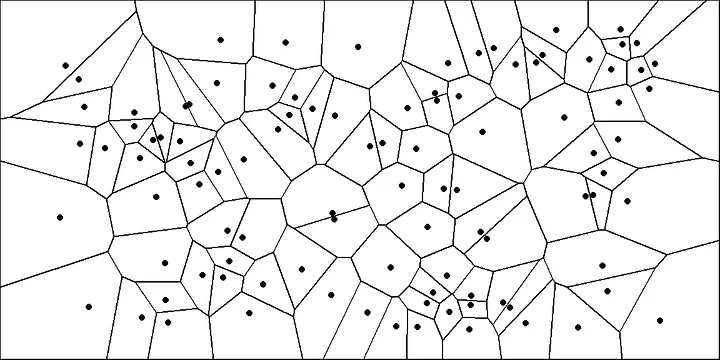
\includegraphics[width=0.4\linewidth]{assets/diagramme_voronoi.png}}%
       {\sources
        Source: \url{towardsdatascience.com}}
\end{figure}

% L'ensemble de ces cellules forment un pavage de plan, appelé \emph{diagramme de Voronoï}.

\end{frame}

%%%%%%%%%%%%%%%%%%%%%%%%%%%%%%%%%%%%%%%%%%%%%%%%
% Deuxième diapo
%%%%%%%%%%%%%%%%%%%%%%%%%%%%%%%%%%%%%%%%%%%%%%%%
\begin{frame}
\frametitle{Représentation}
\framesubtitle{DCEL (Liste d'arêtes doublement chaînées)}

\begin{figure}
    \centering
    \def\stackalignment{r}
    \stackunder{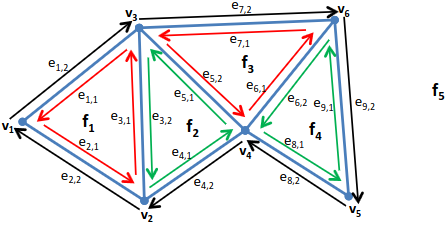
\includegraphics[width=0.6\linewidth]{assets/DCEL.png}}%
           {\sources
        Source: Simon Fraser University}
\end{figure}
\begin{itemize}
    \item Représentation de graphes planaires
    \item Permet de retrouver à partir d'une arête les deux sites des deux faces adjacentes
\end{itemize}
    
\end{frame}

%%%%%%%%%%%%%%%%%%%%%%%%%%%%%%%%%%%%%%%%%%%%%%%%
% Troisième diapo
%%%%%%%%%%%%%%%%%%%%%%%%%%%%%%%%%%%%%%%%%%%%%%%%
\begin{frame}
\frametitle{Algorithme de Fortune}
\begin{columns}
    \begin{column}{6cm}
    \begin{itemize} \itemsep3em
        \item Algorithme avec ligne de balayage (\textit{sweep line}) et ligne de front (\textit{beach line})
        \item \textit{Site events}
        \item \textit{Circle events}
    \end{itemize}
    \end{column}

    \begin{column}{5cm}
            \begin{figure}
                \def\stackalignment{r}
                \stackunder{
                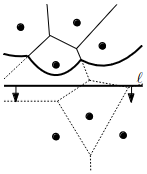
\includegraphics[width=0.7\linewidth]{assets/sweep_line.png}}%
                {\sources Source: Computational Geometry}
            \end{figure}
    \end{column}
\end{columns}
\end{frame}


\begin{frame}{Algorithme de Fortune}
\framesubtitle{\textit{Circle events}}
\begin{figure}
    \centering
    \def\stackalignment{r}
    \stackunder{
        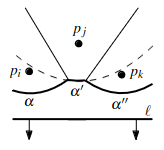
\includegraphics[width=0.4\linewidth]{assets/circle_b.png}
        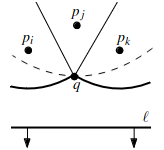
\includegraphics[width=0.4\linewidth]{assets/circle_a.png}}%
       {\sources
        Source: Computational Geometry}
\end{figure}
\end{frame}


\begin{frame}{Un exemple}
\only<1>{\begin{figure}
    \centering
    \def\stackalignment{r}
    \stackunder{
        \includegraphics[width=0.5\linewidth]{assets/wiki_build/frame_06_delay-0.5s.png}}%
       {\sources
        Source: Wikipedia}
\end{figure}}
\only<2>{\begin{figure}
    \centering
    \def\stackalignment{r}
    \stackunder{
        \includegraphics[width=0.5\linewidth]{assets/wiki_build/frame_07_delay-0.5s.png}}%
       {\sources
        Source: Wikipedia}
\end{figure}}
\only<3>{\begin{figure}
    \centering
    \def\stackalignment{r}
    \stackunder{
        \includegraphics[width=0.5\linewidth]{assets/wiki_build/frame_08_delay-0.5s.png}}%
       {\sources
        Source: Wikipedia}
\end{figure}}
\only<4>{\begin{figure}
    \centering
    \def\stackalignment{r}
    \stackunder{
        \includegraphics[width=0.5\linewidth]{assets/wiki_build/frame_09_delay-0.5s.png}}%
       {\sources
        Source: Wikipedia}
\end{figure}}
\only<5>{\begin{figure}
    \centering
    \def\stackalignment{r}
    \stackunder{
        \includegraphics[width=0.5\linewidth]{assets/wiki_build/frame_10_delay-0.5s.png}}%
       {\sources
        Source: Wikipedia}
\end{figure}}
\only<6>{\begin{figure}
    \centering
    \def\stackalignment{r}
    \stackunder{
        \includegraphics[width=0.5\linewidth]{assets/wiki_build/frame_11_delay-0.5s.png}}%
       {\sources
        Source: Wikipedia}
\end{figure}}
\only<7>{\begin{figure}
    \centering
    \def\stackalignment{r}
    \stackunder{
        \includegraphics[width=0.5\linewidth]{assets/wiki_build/frame_12_delay-0.5s.png}}%
       {\sources
        Source: Wikipedia}
\end{figure}}
\only<8>{\begin{figure} 
    \centering
    \def\stackalignment{r}
    \stackunder{
        \includegraphics[width=0.5\linewidth]{assets/wiki_build/frame_13_delay-0.5s.png}}%
       {\sources
        Source: Wikipedia}
\end{figure}}
\end{frame}


%%%%%%%%%%%%%%%%%%%%%%%%%%%%%%%%%%%%%%%%%%%%%%%%
% Quatrième diapo
%%%%%%%%%%%%%%%%%%%%%%%%%%%%%%%%%%%%%%%%%%%%%%%%
\begin{frame}
\frametitle{Algorithme de Fortune}
    \small
    
    \vspace{2pt}
    \begin{algorithmic}
        \State \(T, A, D \gets\) Tas(\(s_1, ..., s_n\)), Arbre(), DCEL()
        \While{\(T\) n'est pas vide}
            \State Retirer de \(T\) l'élément minimal \(e\)
            \If {c'est un \textit{site event}}
                \State \Call{TraitementSiteEvent}{e}
            \Else
                \State a \(\gets \) Recherche dans l'arbre \(A\) de l'arc disparaissant.
                \State \Call{TraitementCircleEvent}{a}
            \EndIf
        \EndWhile
    \normalsize
    \end{algorithmic}
\visible<2->{
\begin{thm}
    L'algorithme de Fortune a une complexité temporelle en \(O(n\log n)\) et spatiale en \(O(n)\).
    Cette complexité est optimale.
\end{thm}}
\end{frame}

%%%%%%%%%%%%%%%%%%%%%%%%%%%%%%%%%%%%%%%%%%%%%%%%
% Cinquième diapo
%%%%%%%%%%%%%%%%%%%%%%%%%%%%%%%%%%%%%%%%%%%%%%%%
\begin{frame}
\frametitle{Mise en oeuvre}
    \begin{figure}
        \centering
        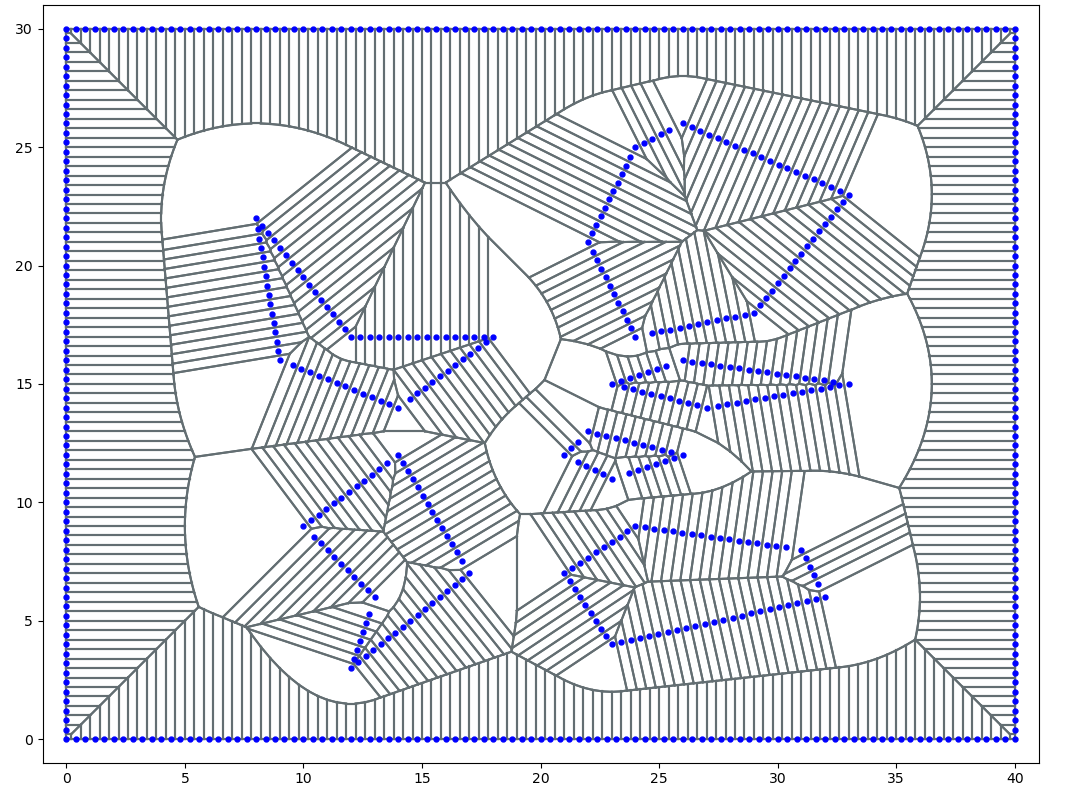
\includegraphics[width=0.8\linewidth]{assets/Voronoi_build.png}
    \end{figure}
\end{frame}

%%%%%%%%%%%%%%%%%%%%%%%%%%%%%%%%%%%%%%%%%%%%%%%%
% Cinquième diapo
%%%%%%%%%%%%%%%%%%%%%%%%%%%%%%%%%%%%%%%%%%%%%%%%
\begin{frame}
    \begin{figure}
        \centering
        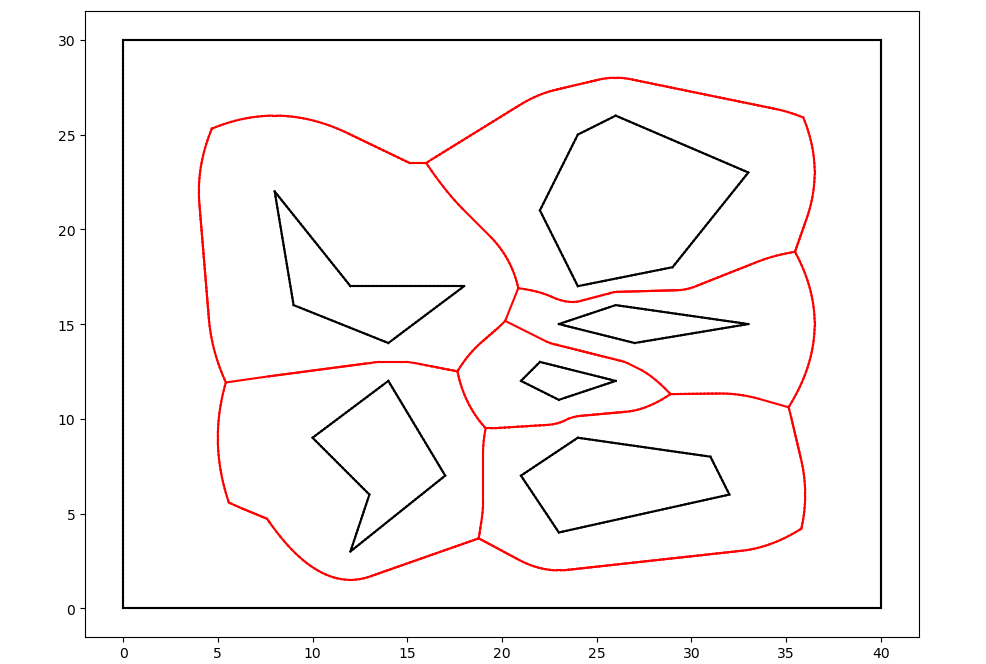
\includegraphics[width=0.7\linewidth]{assets/Voronoi_mapping.png}
    \end{figure}
    \begin{enumerate}
        \item Récupérer les arêtes du diagramme de Voronoï
        \item Conserver uniquement les arêtes "centrales"
        \item Simplifier le graphe
    \end{enumerate}
\end{frame}

%%%%%%%%%%%%%%%%%%%%%%%%%%%%%%%%%%%%%%%%%%%%%%%%
% Cinquième diapo
%%%%%%%%%%%%%%%%%%%%%%%%%%%%%%%%%%%%%%%%%%%%%%%%
\begin{frame}
    \begin{figure}
        \centering
        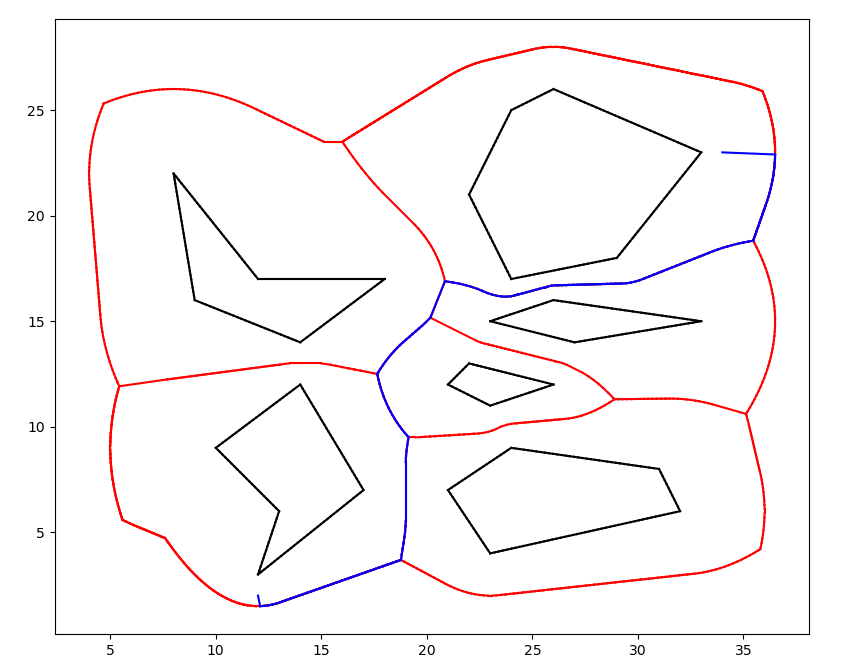
\includegraphics[width=0.65\linewidth]{assets/Voronoi_chemin_highlight.png}
    \end{figure}
    \begin{enumerate}
        \item Chercher les points les plus proches du départ / arrivée
        \item Chercher le chemin dans le graphe simplifié
        \item Reconstituer tous les points intermédiaires
    \end{enumerate}
\end{frame}

%%%%%%%%%%%%%%%%%%%%%%%%%%%%%%%%%%%%%%%%%%%%%%%%
% Fin diapo
%%%%%%%%%%%%%%%%%%%%%%%%%%%%%%%%%%%%%%%%%%%%%%%%
\begin{frame}
\frametitle{Observations de cette approche}
\begin{columns}
    \begin{column}{.4\textwidth}
        \begin{figure}
            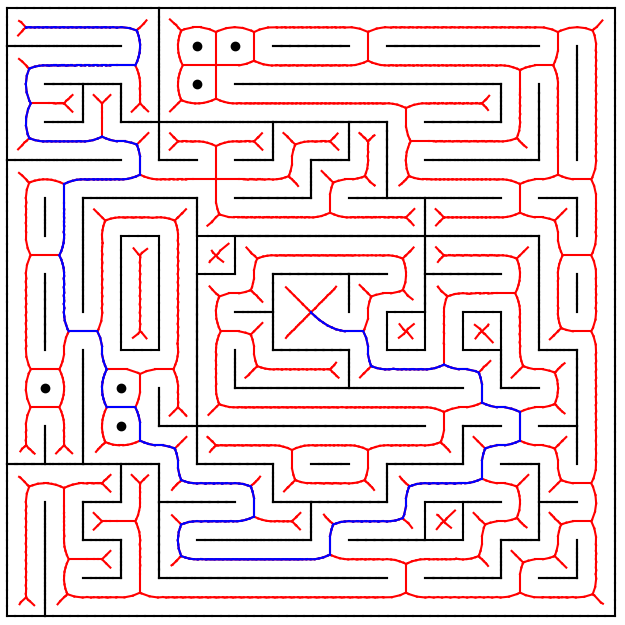
\includegraphics[width=1\linewidth]{assets/BigLabyrinthe.png}
        \end{figure}
    \end{column}
    \begin{column}{.6\textwidth}
        \begin{itemize}
            \item Complexité similaire dans le pire cas: \\ \quad \(O\left (\frac{1}{p^2}\log\frac{1}{p} \right )\)
            \item Ne nécessite pas de fixer de marge à l'avance
        \end{itemize}
    \end{column}
\end{columns}
% \vspace{1em}
\begin{itemize}
    \item Une fois la carte précalculée, la recherche de chemin est instantanée
    \item Les chemins sont plus lisses, virages anticipés
    \item Les chemins évitent mieux les obstacles
\end{itemize}
    \end{frame}